\documentclass{beamer}
\usetheme{Hannover}
\setbeamersize{sidebar width left=0pt}
\usepackage[T1, T2A]{fontenc}
\usepackage[utf8]{inputenc}
\usepackage[russian]{babel}
\usepackage{hyperref}
\usepackage{graphicx}
\graphicspath{ {../Images/} }

\author{Григорий Матюхин}
\date{\today}
\title{Лабораторная работа \textnumero1.}
\subtitle{Установка и конфигурация операционной системы на виртуальную машину}

\begin{document}
  \begin{frame}[plain]
  \titlepage
  \end{frame}
  \section{Цель работы}
  \begin{frame}[plain]
  \frametitle{Цель работы}
  Целью данной работы является приобретение практических навыков установки операционной системы на виртуальную машину, настройки минимально необходимых для дальнейшей работы сервисов.
  \end{frame}

  \section{Результат}
  \begin{frame}[plain]
  \frametitle{Результат}
    Дождитесь загрузки графического окружения и откройте терминал. В окне терминала проанализируйте последовательность загрузки системы, выполнив команду \texttt{dmesg}. Получите следующую информацию.
    \begin{enumerate}
      \item Версия ядра Linux (Linux version).
        \\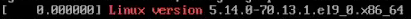
\includegraphics{1.png}\\
      \item Частота процессора (Detected Mhz processor).
        \\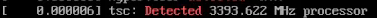
\includegraphics{2.png}\\
      \item Модель процессора (CPU0).
        \\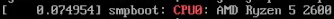
\includegraphics{3.png}\\
      \item Объем доступной оперативной памяти (Memory available).
        \\
\includegraphics{4.png}\\
      \item Тип обнаруженного гипервизора (Hypervisor detected).
        \\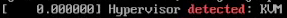
\includegraphics{5.png}\\
      \item Тип файловой системы корневого раздела.
        \\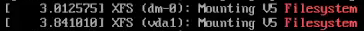
\includegraphics{6.png}\\
      \item Последовательность монтирования файловых систем.
        \\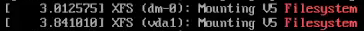
\includegraphics{6.png}\\
    \end{enumerate}
  \end{frame}
  \section{Вывод}
  \begin{frame}[plain]
  \frametitle{Вывод}
    В ходе выполнения данной работы я приобрел практические навыков установки операционной системы на виртуальную машину, настройки минимально необходимых для дальнейшей работы сервисов. 
  \end{frame}
\end{document}
